\ffigbox[\FBwidth]{%
\caption{\centering Graphe \(C_5\) de départ}\label{Fig:exam_blanc_ex_5_1_b}
}{
    \fbox{
        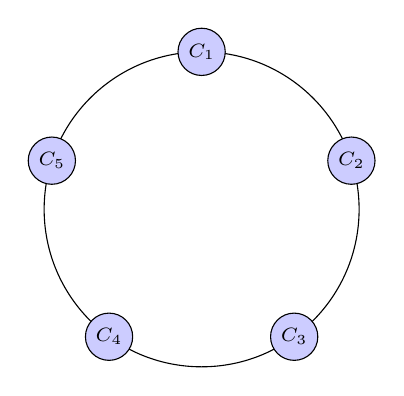
\begin{tikzpicture}[scale=1, main node/.style={circle, draw, fill=blue!20, inner sep=1pt, font=\scriptsize, minimum size=6mm}]
            % le cercle de départ 
            \draw (0, 0) circle [radius=2];
            
            % les sommets initiaux
            \node[main node] (1) at (90:2)  {\(C_1\)};
            \node[main node] (2) at (18:2)  {\(C_2\)};
            \node[main node] (3) at (-54:2) {\(C_3\)};
            \node[main node] (4) at (-126:2){\(C_4\)};
            \node[main node] (5) at (-198:2){\(C_5\)};
            
        \end{tikzpicture}
    }
}